\section{A Parallel Solution}
\label{sec:new}

An inference algorithm can be proposed to the propagation phase in a SPN.
But since they are similar to the inference process using a polynomial network, as noticed in \citep{Peharz:2015tp}, one can use the same propagation algorithm from \citep{Darwiche2009}.
Thus, we show in Figure \ref{fig:alg} one possible algorithm for propagating up and down in a SPN.
This algorithm was taken from \citep{Darwiche2009} Algorithm 34.

\begin{figure}[hbt]
    \begin{center}
    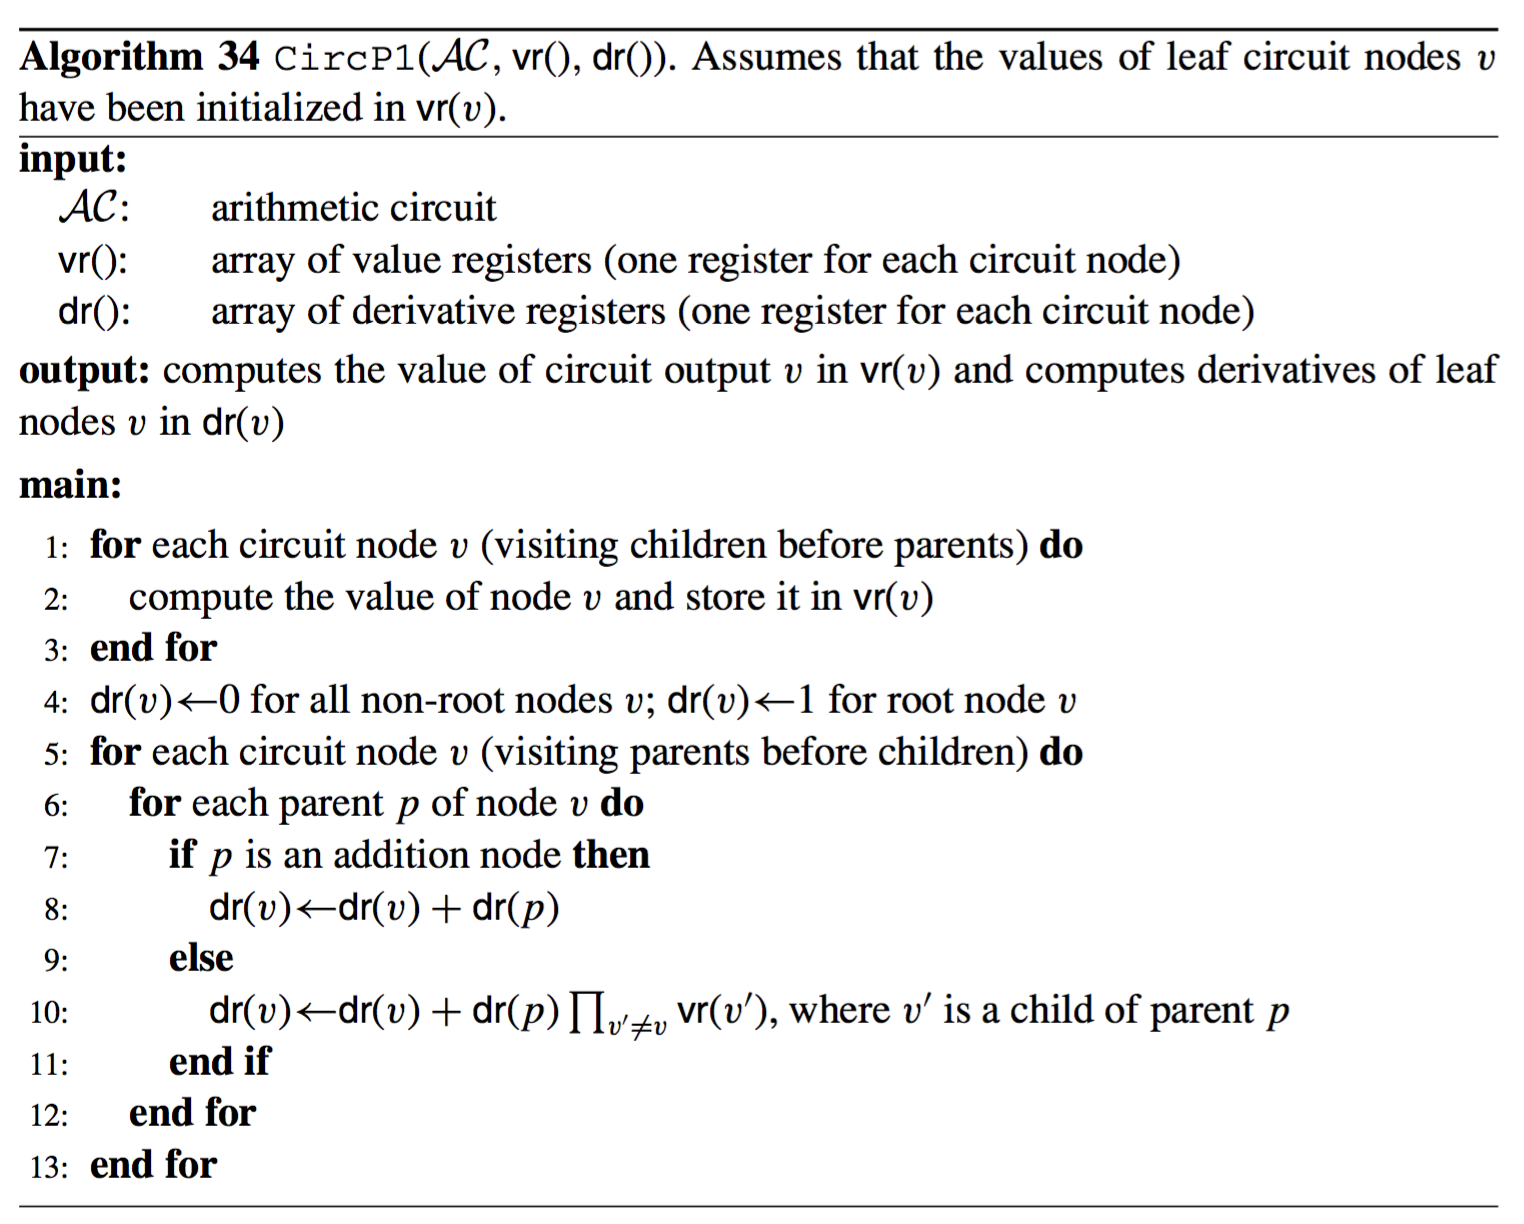
\includegraphics[width=\textwidth]{figures/alg.png}
    \caption{Algorithm \citep{Darwiche2009} for performing inference in a SPN.}
    \label{fig:alg}
    \end{center}
\end{figure}

Parallelizing the Algorithm in Figure \ref{fig:alg} can be simply done by parallelizing the outer for-loop, in line 5.
The main idea here is that, in the SPN of Figure \ref{fig:spn}, one can compute the values of all nodes at each layer.
For instance, the first product layer can be computed all at once.
Next, the sum layer can again be computed all at once, and so on.
This is only possible since each layer does not require input values from its internal nodes.

There are few concerns when parallelizing the inference process.
The first one is regarding layers that intersect the DAG later on and not from the top.
For instance, consider the SPN in Figure \ref{fig:spn}.
The layer involving nodes $\lambda_a$ and $\theta_a$ has to wait for the other children of its parent.
This can be safely done by imposing a limitation at each layer: only compute its values when the previously layer is done.
The second possible issue is regarding shared variables within each layer.
For instance, variable $\lambda_b$ is involves in two multiplication at the bottom layer.
Since we are only considering SPNs with real value nodes, this can be safely computed by creating a copy of that shared node value.
In case where nodes are also functions, a more sophisticated solution is required.
But this issue is out of the scope of this paper.
